% Options for packages loaded elsewhere
\PassOptionsToPackage{unicode}{hyperref}
\PassOptionsToPackage{hyphens}{url}
%
\documentclass[
  10pt,
  ignorenonframetext,
]{beamer}
\usepackage{pgfpages}
\setbeamertemplate{caption}[numbered]
\setbeamertemplate{caption label separator}{: }
\setbeamercolor{caption name}{fg=normal text.fg}
\beamertemplatenavigationsymbolsempty
% Prevent slide breaks in the middle of a paragraph
\widowpenalties 1 10000
\raggedbottom
\setbeamertemplate{part page}{
  \centering
  \begin{beamercolorbox}[sep=16pt,center]{part title}
    \usebeamerfont{part title}\insertpart\par
  \end{beamercolorbox}
}
\setbeamertemplate{section page}{
  \centering
  \begin{beamercolorbox}[sep=12pt,center]{part title}
    \usebeamerfont{section title}\insertsection\par
  \end{beamercolorbox}
}
\setbeamertemplate{subsection page}{
  \centering
  \begin{beamercolorbox}[sep=8pt,center]{part title}
    \usebeamerfont{subsection title}\insertsubsection\par
  \end{beamercolorbox}
}
\AtBeginPart{
  \frame{\partpage}
}
\AtBeginSection{
  \ifbibliography
  \else
    \frame{\sectionpage}
  \fi
}
\AtBeginSubsection{
  \frame{\subsectionpage}
}
\usepackage{amsmath,amssymb}
\usepackage{lmodern}
\usepackage{ifxetex,ifluatex}
\ifnum 0\ifxetex 1\fi\ifluatex 1\fi=0 % if pdftex
  \usepackage[T1]{fontenc}
  \usepackage[utf8]{inputenc}
  \usepackage{textcomp} % provide euro and other symbols
\else % if luatex or xetex
  \usepackage{unicode-math}
  \defaultfontfeatures{Scale=MatchLowercase}
  \defaultfontfeatures[\rmfamily]{Ligatures=TeX,Scale=1}
\fi
\usecolortheme{beaver}
% Use upquote if available, for straight quotes in verbatim environments
\IfFileExists{upquote.sty}{\usepackage{upquote}}{}
\IfFileExists{microtype.sty}{% use microtype if available
  \usepackage[]{microtype}
  \UseMicrotypeSet[protrusion]{basicmath} % disable protrusion for tt fonts
}{}
\makeatletter
\@ifundefined{KOMAClassName}{% if non-KOMA class
  \IfFileExists{parskip.sty}{%
    \usepackage{parskip}
  }{% else
    \setlength{\parindent}{0pt}
    \setlength{\parskip}{6pt plus 2pt minus 1pt}}
}{% if KOMA class
  \KOMAoptions{parskip=half}}
\makeatother
\usepackage{xcolor}
\IfFileExists{xurl.sty}{\usepackage{xurl}}{} % add URL line breaks if available
\IfFileExists{bookmark.sty}{\usepackage{bookmark}}{\usepackage{hyperref}}
\hypersetup{
  pdftitle={Manejo de datos en R (I)},
  pdfauthor={Introducción a la Línea de Comandos para Análisis Bioinformáticos},
  hidelinks,
  pdfcreator={LaTeX via pandoc}}
\urlstyle{same} % disable monospaced font for URLs
\newif\ifbibliography
\usepackage{color}
\usepackage{fancyvrb}
\newcommand{\VerbBar}{|}
\newcommand{\VERB}{\Verb[commandchars=\\\{\}]}
\DefineVerbatimEnvironment{Highlighting}{Verbatim}{commandchars=\\\{\}}
% Add ',fontsize=\small' for more characters per line
\usepackage{framed}
\definecolor{shadecolor}{RGB}{248,248,248}
\newenvironment{Shaded}{\begin{snugshade}}{\end{snugshade}}
\newcommand{\AlertTok}[1]{\textcolor[rgb]{0.94,0.16,0.16}{#1}}
\newcommand{\AnnotationTok}[1]{\textcolor[rgb]{0.56,0.35,0.01}{\textbf{\textit{#1}}}}
\newcommand{\AttributeTok}[1]{\textcolor[rgb]{0.77,0.63,0.00}{#1}}
\newcommand{\BaseNTok}[1]{\textcolor[rgb]{0.00,0.00,0.81}{#1}}
\newcommand{\BuiltInTok}[1]{#1}
\newcommand{\CharTok}[1]{\textcolor[rgb]{0.31,0.60,0.02}{#1}}
\newcommand{\CommentTok}[1]{\textcolor[rgb]{0.56,0.35,0.01}{\textit{#1}}}
\newcommand{\CommentVarTok}[1]{\textcolor[rgb]{0.56,0.35,0.01}{\textbf{\textit{#1}}}}
\newcommand{\ConstantTok}[1]{\textcolor[rgb]{0.00,0.00,0.00}{#1}}
\newcommand{\ControlFlowTok}[1]{\textcolor[rgb]{0.13,0.29,0.53}{\textbf{#1}}}
\newcommand{\DataTypeTok}[1]{\textcolor[rgb]{0.13,0.29,0.53}{#1}}
\newcommand{\DecValTok}[1]{\textcolor[rgb]{0.00,0.00,0.81}{#1}}
\newcommand{\DocumentationTok}[1]{\textcolor[rgb]{0.56,0.35,0.01}{\textbf{\textit{#1}}}}
\newcommand{\ErrorTok}[1]{\textcolor[rgb]{0.64,0.00,0.00}{\textbf{#1}}}
\newcommand{\ExtensionTok}[1]{#1}
\newcommand{\FloatTok}[1]{\textcolor[rgb]{0.00,0.00,0.81}{#1}}
\newcommand{\FunctionTok}[1]{\textcolor[rgb]{0.00,0.00,0.00}{#1}}
\newcommand{\ImportTok}[1]{#1}
\newcommand{\InformationTok}[1]{\textcolor[rgb]{0.56,0.35,0.01}{\textbf{\textit{#1}}}}
\newcommand{\KeywordTok}[1]{\textcolor[rgb]{0.13,0.29,0.53}{\textbf{#1}}}
\newcommand{\NormalTok}[1]{#1}
\newcommand{\OperatorTok}[1]{\textcolor[rgb]{0.81,0.36,0.00}{\textbf{#1}}}
\newcommand{\OtherTok}[1]{\textcolor[rgb]{0.56,0.35,0.01}{#1}}
\newcommand{\PreprocessorTok}[1]{\textcolor[rgb]{0.56,0.35,0.01}{\textit{#1}}}
\newcommand{\RegionMarkerTok}[1]{#1}
\newcommand{\SpecialCharTok}[1]{\textcolor[rgb]{0.00,0.00,0.00}{#1}}
\newcommand{\SpecialStringTok}[1]{\textcolor[rgb]{0.31,0.60,0.02}{#1}}
\newcommand{\StringTok}[1]{\textcolor[rgb]{0.31,0.60,0.02}{#1}}
\newcommand{\VariableTok}[1]{\textcolor[rgb]{0.00,0.00,0.00}{#1}}
\newcommand{\VerbatimStringTok}[1]{\textcolor[rgb]{0.31,0.60,0.02}{#1}}
\newcommand{\WarningTok}[1]{\textcolor[rgb]{0.56,0.35,0.01}{\textbf{\textit{#1}}}}
\usepackage{graphicx}
\makeatletter
\def\maxwidth{\ifdim\Gin@nat@width>\linewidth\linewidth\else\Gin@nat@width\fi}
\def\maxheight{\ifdim\Gin@nat@height>\textheight\textheight\else\Gin@nat@height\fi}
\makeatother
% Scale images if necessary, so that they will not overflow the page
% margins by default, and it is still possible to overwrite the defaults
% using explicit options in \includegraphics[width, height, ...]{}
\setkeys{Gin}{width=\maxwidth,height=\maxheight,keepaspectratio}
% Set default figure placement to htbp
\makeatletter
\def\fps@figure{htbp}
\makeatother
\setlength{\emergencystretch}{3em} % prevent overfull lines
\providecommand{\tightlist}{%
  \setlength{\itemsep}{0pt}\setlength{\parskip}{0pt}}
\setcounter{secnumdepth}{-\maxdimen} % remove section numbering
\usepackage{tikz}
\usepackage{graphicx}
\usetikzlibrary{calc}
\usepackage{pgfplots}
\usepackage{environ}
\useoutertheme{miniframes}
\usepackage{ragged2e}
\useinnertheme{circles}
\setbeameroption{hide notes}
\ifluatex
  \usepackage{selnolig}  % disable illegal ligatures
\fi

\title{Manejo de datos en R (I)}
\author{Introducción a la Línea de Comandos para Análisis
Bioinformáticos}
\date{10 de Agosto, 2021}

\begin{document}
\frame{\titlepage}

\hypertarget{que-vamos-a-hacer}{%
\section{Que vamos a hacer?}\label{que-vamos-a-hacer}}

\begin{frame}{Manejo de datos y análisis reproducible}
\protect\hypertarget{manejo-de-datos-y-anuxe1lisis-reproducible}{}
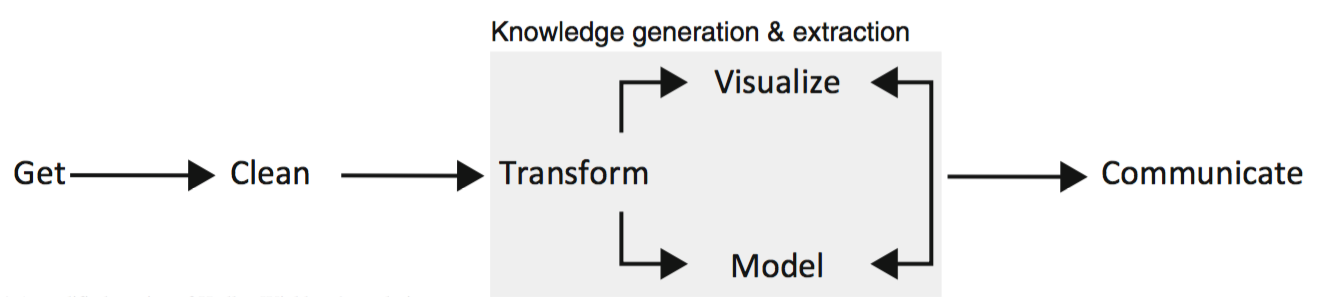
\includegraphics{../../imgs/analytic_process.png}

\vspace{60pt}

\raggedleft \small \href{http://93.174.95.29/_ads/6F902E466A32011DD94E2B6EEE505F9F}{Data
Wrangling with R (Boehmke, 2016)}
\end{frame}

\begin{frame}{Análisis reproducible en R}
\protect\hypertarget{anuxe1lisis-reproducible-en-r}{}
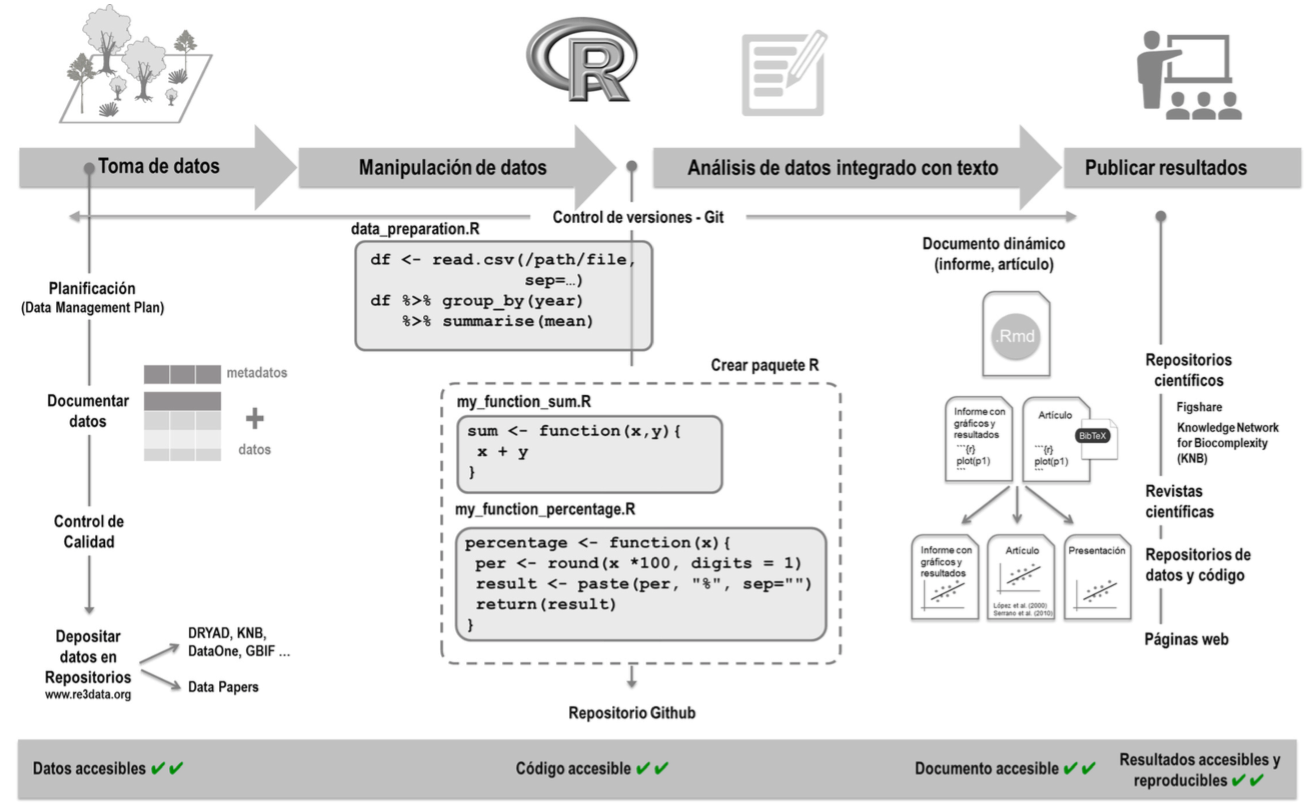
\includegraphics{../../imgs/analytic_process_R.png}

\raggedleft \small \href{https://revistaecosistemas.net/index.php/ecosistemas/article/view/1178}{Ciencia
reproducible: qué, por qué, cómo (Rodríguez-Sánchez et al., 2016)}
\end{frame}

\begin{frame}{Manejo de datos}
\protect\hypertarget{manejo-de-datos}{}
\begin{itemize}
\tightlist
\item
  \textbf{\emph{Data wrangling}}: es el proceso mediante el cual
  modificamos datos iniciales con el fin de analizarlos. \vspace{15pt}
\item
  Incluye la edición, el filtrado, la obtención de nuevos valores y más.
  \vspace{15pt}
\item
  \emph{``In our experience, the tasks of exploratory data mining and
  data cleaning constitute 80\% of the effort that determines 80\% of
  the value of the ultimate data mining results. (\ldots)''}.
  \textbackslash{} \textbf{Dasu \& Johnson.} \emph{Exploratory Data
  Mining and Data Cleaning} (2003).
\end{itemize}
\end{frame}

\begin{frame}{Estructura de las clases}
\protect\hypertarget{estructura-de-las-clases}{}
\begin{itemize}
\item
  Teórico/práctico. \vspace{12pt}
\item
  Práctico 11: repaso de loops y armado de funciones en R

  \begin{itemize}
  \tightlist
  \item
    accionar sobre los datos para transformarlos: funciones
  \item
    realizar acciones repetitivas: loops \vspace{12pt}
  \end{itemize}
\item
  Práctico 12: manejo de datos con paquetes de la librería
  \textbf{tidyverse}.

  \begin{itemize}
  \tightlist
  \item
    filtrado y edición de datos
  \item
    visualización de los datos
  \end{itemize}
\end{itemize}
\end{frame}

\hypertarget{breve-repaso-de-r}{%
\section{Breve repaso de R}\label{breve-repaso-de-r}}

\begin{frame}{Breve repaso}
\protect\hypertarget{breve-repaso}{}
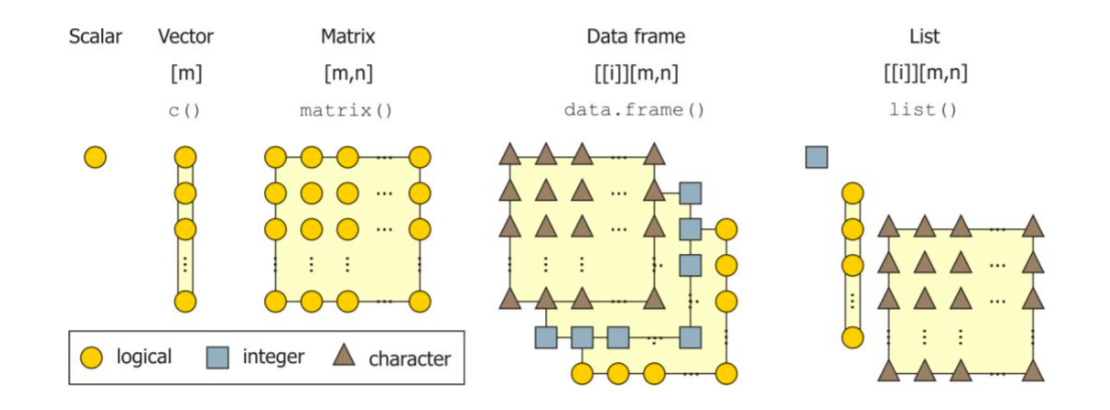
\includegraphics{../../imgs/r_tipos_datos.png}

\vspace{50pt}

\raggedleft \small \href{https://hal.archives-ouvertes.fr/hal-01846155/document}{A
practical guide to the R package Luminescence (Dietze et al., 2013)}
\end{frame}

\begin{frame}{Breve repaso}
\protect\hypertarget{breve-repaso-1}{}
\begin{center}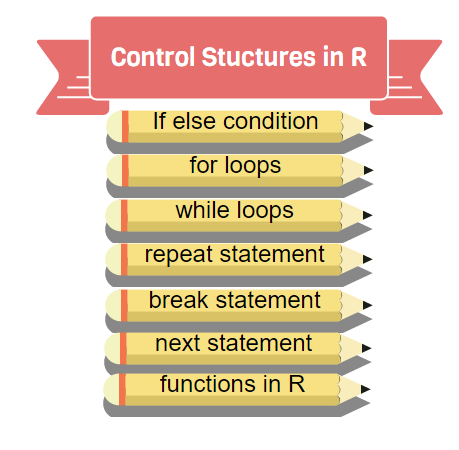
\includegraphics[width=0.6\linewidth]{../../imgs/control_structures+in+R} \end{center}

\raggedleft \small \href{https://www.r-bloggers.com/control-structures-loops-in-r/}{Control
Structures in R (R-Bloggers)}
\end{frame}

\begin{frame}{Breve repaso}
\protect\hypertarget{breve-repaso-2}{}
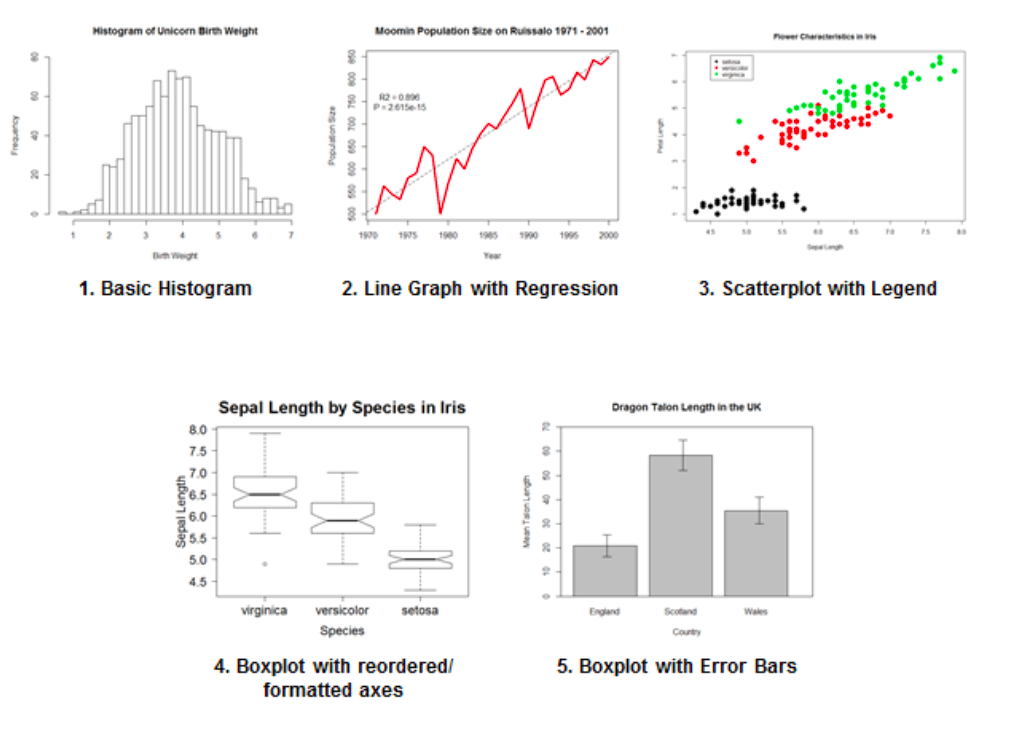
\includegraphics{../../imgs/r_base_graphs.png} \vspace{15pt}
\raggedleft \small \href{https://rpubs.com/SusanEJohnston/7953}{R Base
Graphs: an Idiot's Guide}
\end{frame}

\hypertarget{funciones-en-r}{%
\section{Funciones en R}\label{funciones-en-r}}

\begin{frame}{Funciones: una parte central de R}
\protect\hypertarget{funciones-una-parte-central-de-r}{}
\begin{itemize}
\item
  Qué es una función? Un conjunto de \textbf{operaciones} definidas que
  toman \textbf{argumentos} para dar un resultado.
\item
  R Es un lenguaje de programación en base a funciones: casi todo lo que
  hacemos las utiliza.

  \begin{itemize}
  \tightlist
  \item
    Otros lenguajes operan de forma diferente.
  \end{itemize}
\item
  Ventajas

  \begin{itemize}
  \tightlist
  \item
    Le podemos dar nombre descriptivo
  \item
    Nos ahorramos copiar y pegar codigo varias veces (y errar en el
    proceso)
  \item
    Si hay que cambiar algo, es solo cambiar la funcion
  \end{itemize}
\item
  Las funciones en R salen de muchos lados:

  \begin{itemize}
  \tightlist
  \item
    R tiene funciones que vienen incorporadas por defecto
  \item
    Utilizando librerías obtenemos nuevas funciones (como las de
    \textbf{seqinr}, por ejemplo)
  \item
    Nosotros podemos hacer nuestras propias funciones
  \end{itemize}
\end{itemize}
\end{frame}

\begin{frame}[fragile]{Ejemplo de una función}
\protect\hypertarget{ejemplo-de-una-funciuxf3n}{}
En la clase pasada operaron sobre variables que alojaban secuencias,
utilizando funciones como la funcion \textbf{GC} de la libreria seqinr
\vspace{15pt}

\begin{Shaded}
\begin{Highlighting}[]
\FunctionTok{library}\NormalTok{(seqinr)}

\NormalTok{seqinr}\SpecialCharTok{::}\FunctionTok{GC}\NormalTok{(secuencia)}
\end{Highlighting}
\end{Shaded}

\begin{verbatim}
## [1] 0.5454545
\end{verbatim}

\vspace{15pt}

Como funciona esto?
\end{frame}

\begin{frame}{Componentes de una función}
\protect\hypertarget{componentes-de-una-funciuxf3n}{}
\begin{itemize}
\item
  \textbf{cuerpo}: el código que define a la función \vspace{12pt}
\item
  \textbf{formales}: la lista de argumentos que controlan cómo se llama
  a la función \vspace{12pt}
\item
  \textbf{ambiente}: el ``mapa'' de la locación de las variables de la
  función

  \begin{itemize}
  \tightlist
  \item
    Es la unica que se define implicitamente, dependiendo de donde uno
    define la funcion
  \end{itemize}
\end{itemize}
\end{frame}

\begin{frame}[fragile]{Componentes de una función}
\protect\hypertarget{componentes-de-una-funciuxf3n-1}{}
\begin{Shaded}
\begin{Highlighting}[]
\FunctionTok{library}\NormalTok{(seqinr)}

\FunctionTok{body}\NormalTok{(seqinr}\SpecialCharTok{::}\NormalTok{GC)}
\end{Highlighting}
\end{Shaded}

\begin{verbatim}
## {
##     if (length(seq) == 1 && is.na(seq)) 
##         return(NA)
##     if (nchar(seq[1]) > 1) 
##         stop("sequence is not a vector of chars")
...
\end{verbatim}

Toda funcion tiene que especificar como hace lo que hace en algun
lugar\ldots{}
\end{frame}

\begin{frame}[fragile]{Componentes de una función}
\protect\hypertarget{componentes-de-una-funciuxf3n-2}{}
\begin{Shaded}
\begin{Highlighting}[]
\FunctionTok{library}\NormalTok{(seqinr)}

\FunctionTok{formals}\NormalTok{(seqinr}\SpecialCharTok{::}\NormalTok{GC)}
\end{Highlighting}
\end{Shaded}

\begin{verbatim}
## $seq
## 
## 
## $forceToLower
## [1] TRUE
## 
## $exact
## [1] FALSE
## 
## $NA.GC
...
\end{verbatim}

Los argumentos tambien se alojan en algun lugar.
\end{frame}

\begin{frame}[fragile]{Componentes de una función}
\protect\hypertarget{componentes-de-una-funciuxf3n-3}{}
\begin{Shaded}
\begin{Highlighting}[]
\FunctionTok{library}\NormalTok{(seqinr)}

\FunctionTok{environment}\NormalTok{(seqinr}\SpecialCharTok{::}\NormalTok{GC)}
\end{Highlighting}
\end{Shaded}

\begin{verbatim}
## <environment: namespace:seqinr>
\end{verbatim}

La funcion va a buscar, en primer lugar, variables definidas en el
ambiente ``seqinr''.
\end{frame}

\begin{frame}[fragile]{Definición de funciones}
\protect\hypertarget{definiciuxf3n-de-funciones}{}
Nosotros podemos hacer nuestras propias funciones, a medida de lo que
necesitamos. \vspace{15pt}

\begin{Shaded}
\begin{Highlighting}[]
\NormalTok{mi\_funcion }\OtherTok{=} \ControlFlowTok{function}\NormalTok{(argumento\_1, argumento\_2, ...)\{}
\CommentTok{\#\textless{}{-}\textgreater{} el indentado no es obligatorio, pero ayuda a leer  }
  \CommentTok{\# en este bloque suceden operaciones con argumento\_1}
\NormalTok{  ...}
  \CommentTok{\# en este bloque suceden operaciones con argumento\_2}
\NormalTok{  ...}
  \CommentTok{\# se devuelve algo como resultado de aplicar}
  \CommentTok{\# la funcion a los argumentos}
  \FunctionTok{return}\NormalTok{(una\_variable\_nueva) }
\NormalTok{\} }\CommentTok{\# una linea sola para este parentesis ayuda a leer}
\end{Highlighting}
\end{Shaded}
\end{frame}

\begin{frame}[fragile]{Definición de funciones}
\protect\hypertarget{definiciuxf3n-de-funciones-1}{}
Hagamos una funcion que opere con dos numeros cualesquiera, \emph{x} e
\emph{y}. \vspace{15pt}

\begin{Shaded}
\begin{Highlighting}[]
\NormalTok{eleva\_y\_resta }\OtherTok{=} \ControlFlowTok{function}\NormalTok{(x,y)\{}
\NormalTok{  resultado }\OtherTok{=}\NormalTok{ x}\SpecialCharTok{\^{}}\DecValTok{2} \SpecialCharTok{{-}}\NormalTok{ y}\SpecialCharTok{\^{}}\DecValTok{2}
  \FunctionTok{return}\NormalTok{(resultado)}
\NormalTok{\}}
\end{Highlighting}
\end{Shaded}
\end{frame}

\begin{frame}[fragile]{Definición de funciones}
\protect\hypertarget{definiciuxf3n-de-funciones-2}{}
Hagamos una funcion que opere con dos numeros cualesquiera, \emph{x} e
\emph{y}. \vspace{15pt}

\begin{Shaded}
\begin{Highlighting}[]
\NormalTok{eleva\_y\_resta }\OtherTok{=} \ControlFlowTok{function}\NormalTok{(x,y)\{}
\NormalTok{  resultado }\OtherTok{=}\NormalTok{ x}\SpecialCharTok{\^{}}\DecValTok{2} \SpecialCharTok{{-}}\NormalTok{ y}\SpecialCharTok{\^{}}\DecValTok{2}
  \FunctionTok{return}\NormalTok{(resultado)}
\NormalTok{\}}

\FunctionTok{eleva\_y\_resta}\NormalTok{(}\DecValTok{2}\NormalTok{,}\DecValTok{3}\NormalTok{)}
\end{Highlighting}
\end{Shaded}

\begin{verbatim}
## [1] -5
\end{verbatim}

\vspace{15pt}

Puedo pasar argumentos sin especificarlos explicitamente. Se interpreta
el valor de cada argumento segun el orden de entrada.
\end{frame}

\begin{frame}[fragile]{Definición de funciones}
\protect\hypertarget{definiciuxf3n-de-funciones-3}{}
Hagamos una funcion que opere con dos numeros cualesquiera, \emph{x} e
\emph{y}. \vspace{15pt}

\begin{Shaded}
\begin{Highlighting}[]
\NormalTok{eleva\_y\_resta }\OtherTok{=} \ControlFlowTok{function}\NormalTok{(x,y)\{}
\NormalTok{  resultado }\OtherTok{=}\NormalTok{ x}\SpecialCharTok{\^{}}\DecValTok{2} \SpecialCharTok{{-}}\NormalTok{ y}\SpecialCharTok{\^{}}\DecValTok{2}
  \FunctionTok{return}\NormalTok{(resultado)}
\NormalTok{\}}

\FunctionTok{eleva\_y\_resta}\NormalTok{(}\AttributeTok{y =} \DecValTok{2}\NormalTok{, }\AttributeTok{x =}\DecValTok{3}\NormalTok{)}
\end{Highlighting}
\end{Shaded}

\begin{verbatim}
## [1] 5
\end{verbatim}
\end{frame}

\begin{frame}[fragile]{Definición de funciones}
\protect\hypertarget{definiciuxf3n-de-funciones-4}{}
Hagamos una funcion que opere con dos numeros cualesquiera, \emph{x} e
\emph{y}. \vspace{15pt}

\begin{Shaded}
\begin{Highlighting}[]
\NormalTok{eleva\_y\_resta }\OtherTok{=} \ControlFlowTok{function}\NormalTok{(x,y)\{}
\NormalTok{  resultado }\OtherTok{=}\NormalTok{ x}\SpecialCharTok{\^{}}\DecValTok{2} \SpecialCharTok{{-}}\NormalTok{ y}\SpecialCharTok{\^{}}\DecValTok{2}
  \FunctionTok{return}\NormalTok{(resultado)}
\NormalTok{\}}

\FunctionTok{eleva\_y\_resta}\NormalTok{(}\AttributeTok{y =} \DecValTok{2}\NormalTok{)}
\end{Highlighting}
\end{Shaded}

\begin{verbatim}
## Error in eleva_y_resta(y = 2): argument "x" is missing, with no default
\end{verbatim}

\vspace{15pt}

Si un argumento utilizado en la funcion no tiene un valor asignado,
sucede un error!
\end{frame}

\begin{frame}[fragile]{Las funciones estan en todos lados\ldots{}}
\protect\hypertarget{las-funciones-estan-en-todos-lados}{}
"Para entender el computo en \emph{R}, dos sloganes son utiles:

\begin{itemize}
\item
  Todo lo que existe es un objeto.
\item
  Todo sucede llamando a una funcion."
\end{itemize}

\hfill --- Joe Chambers

\vspace{12pt}

En R usamos funciones hasta sin saberlo

\begin{Shaded}
\begin{Highlighting}[]
\NormalTok{un\_vector }\OtherTok{=} \FunctionTok{c}\NormalTok{(}\DecValTok{1}\NormalTok{, }\DecValTok{4}\NormalTok{, }\DecValTok{6}\NormalTok{) }\CommentTok{\# una funcion me permitio hacer esto}
\NormalTok{un\_vector[}\DecValTok{1}\NormalTok{] }\CommentTok{\# y tambien una funcion me permitio hacer esto}
\end{Highlighting}
\end{Shaded}

\begin{verbatim}
## [1] 1
\end{verbatim}

\vspace{12pt}

Tanto \textbf{c}, como \textbf{=}, como \textbf{{[}} son funciones,
aunque no lo parezcan.
\end{frame}

\begin{frame}[fragile]{Las funciones estan en todos lados\ldots{}}
\protect\hypertarget{las-funciones-estan-en-todos-lados-1}{}
\begin{Shaded}
\begin{Highlighting}[]
\StringTok{\textasciigrave{}}\AttributeTok{[}\StringTok{\textasciigrave{}}
\end{Highlighting}
\end{Shaded}

\begin{verbatim}
## .Primitive("[")
\end{verbatim}

\begin{Shaded}
\begin{Highlighting}[]
\StringTok{\textasciigrave{}}\AttributeTok{for}\StringTok{\textasciigrave{}}
\end{Highlighting}
\end{Shaded}

\begin{verbatim}
## .Primitive("for")
\end{verbatim}

\begin{Shaded}
\begin{Highlighting}[]
\StringTok{\textasciigrave{}}\AttributeTok{c}\StringTok{\textasciigrave{}}
\end{Highlighting}
\end{Shaded}

\begin{verbatim}
## function (...)  .Primitive("c")
\end{verbatim}

\vspace{12pt}

Son funciones llamadas \emph{primitivas}. Estan escritas en el lenguaje
C de programacion, y no podemos acceder a su codigo.
\end{frame}

\hypertarget{loops-en-r}{%
\section{Loops en R}\label{loops-en-r}}

\begin{frame}[fragile]{For loop (abstracto)}
\protect\hypertarget{for-loop-abstracto}{}
En las clases anteriores vieron estructuras del estilo: \vspace{15pt}

\begin{Shaded}
\begin{Highlighting}[]
\CommentTok{\# for loop}

\NormalTok{un\_vector }\OtherTok{=}\NormalTok{ ...}
\ControlFlowTok{for}\NormalTok{ (i }\ControlFlowTok{in}\NormalTok{ \_\_\_\_) \{}
\NormalTok{  ...}
\NormalTok{  ... un\_vector[i] ....}
\NormalTok{  ...}
\NormalTok{\}}
\end{Highlighting}
\end{Shaded}

\vspace{15pt}

En R los loops utilizan indices para acceder a elementos de un
vector/lista
\end{frame}

\begin{frame}{For loop (la logica)}
\protect\hypertarget{for-loop-la-logica}{}
\begin{center}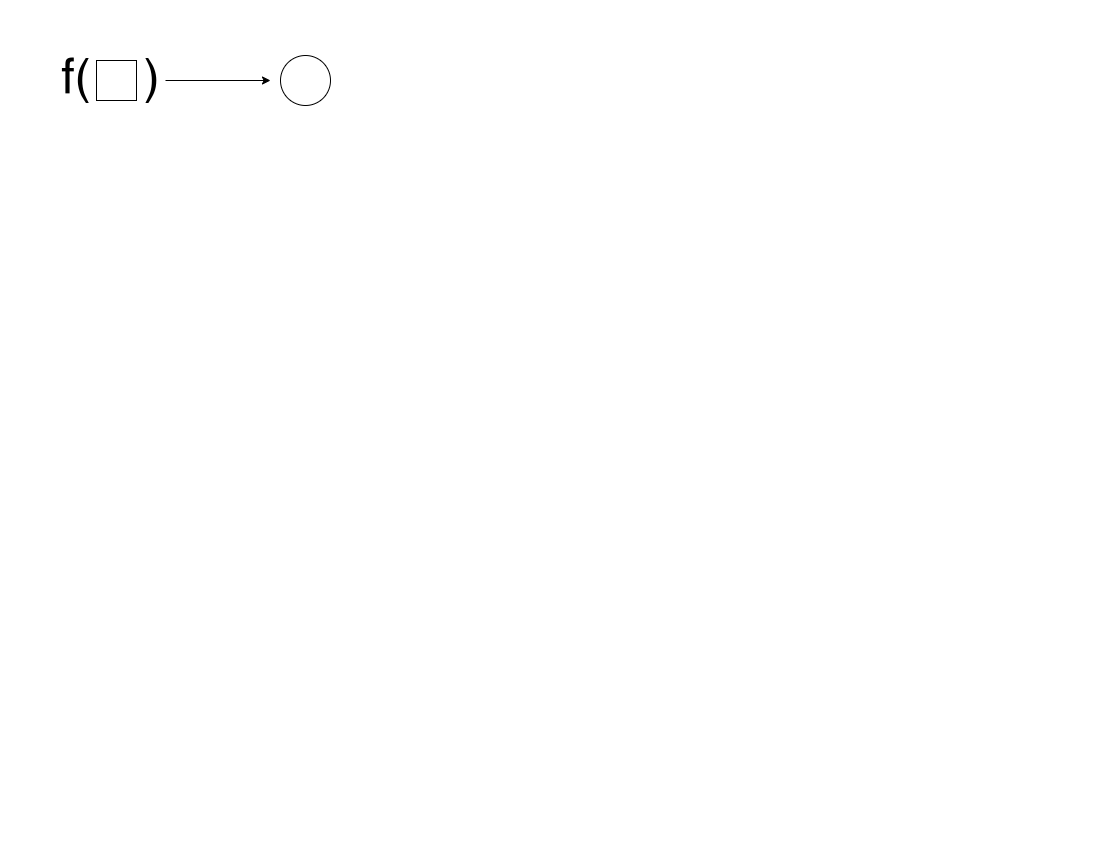
\includegraphics[width=0.9\linewidth]{images/explicando_forloops_en_r_0a} \end{center}
\end{frame}

\begin{frame}{For loop (la logica)}
\protect\hypertarget{for-loop-la-logica-1}{}
\begin{center}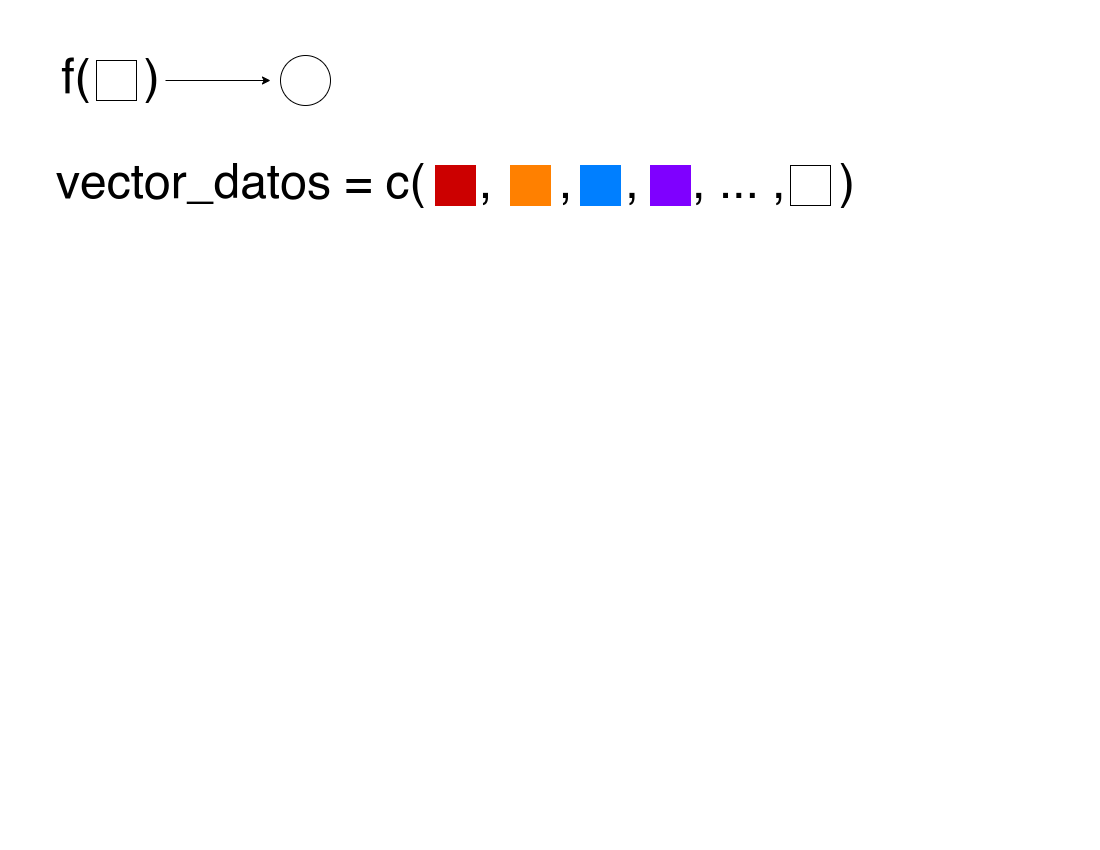
\includegraphics[width=0.9\linewidth]{images/explicando_forloops_en_r_0b} \end{center}
\end{frame}

\begin{frame}{For loop (la logica)}
\protect\hypertarget{for-loop-la-logica-2}{}
\begin{center}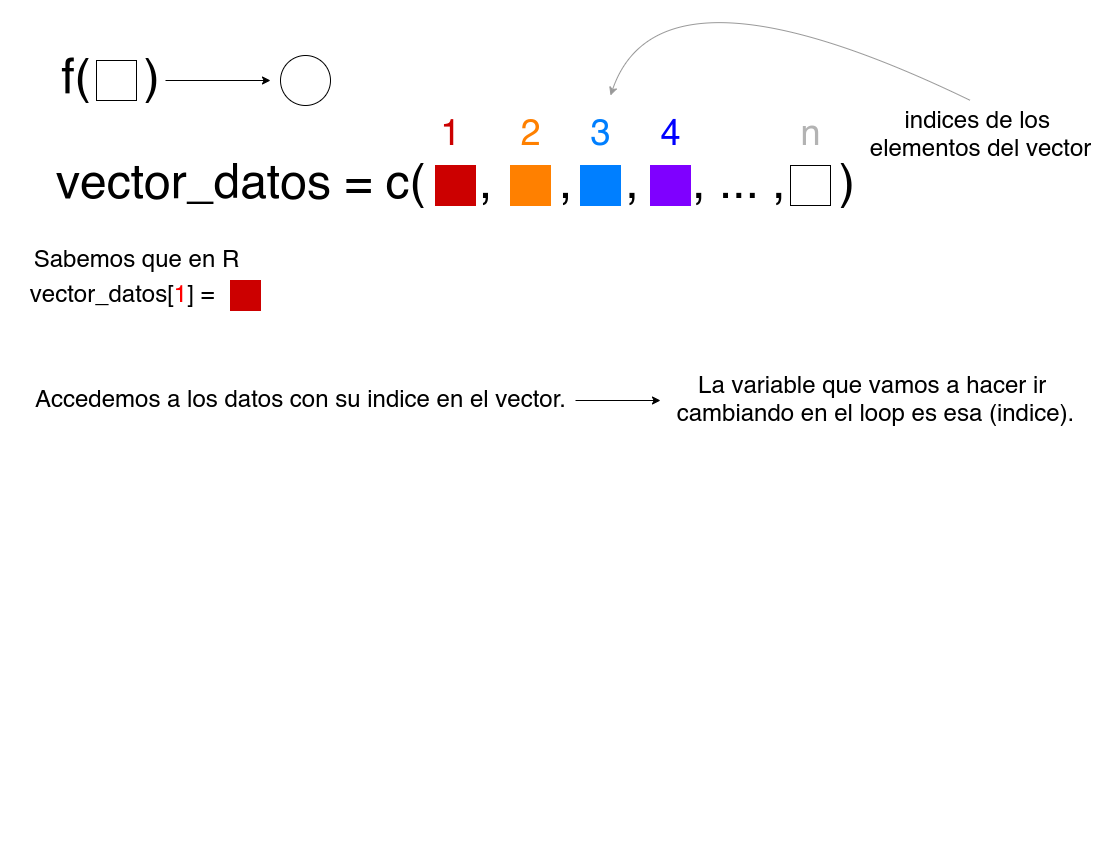
\includegraphics[width=0.9\linewidth]{images/explicando_forloops_en_r_0c} \end{center}
\end{frame}

\begin{frame}{For loop (la logica)}
\protect\hypertarget{for-loop-la-logica-3}{}
\begin{center}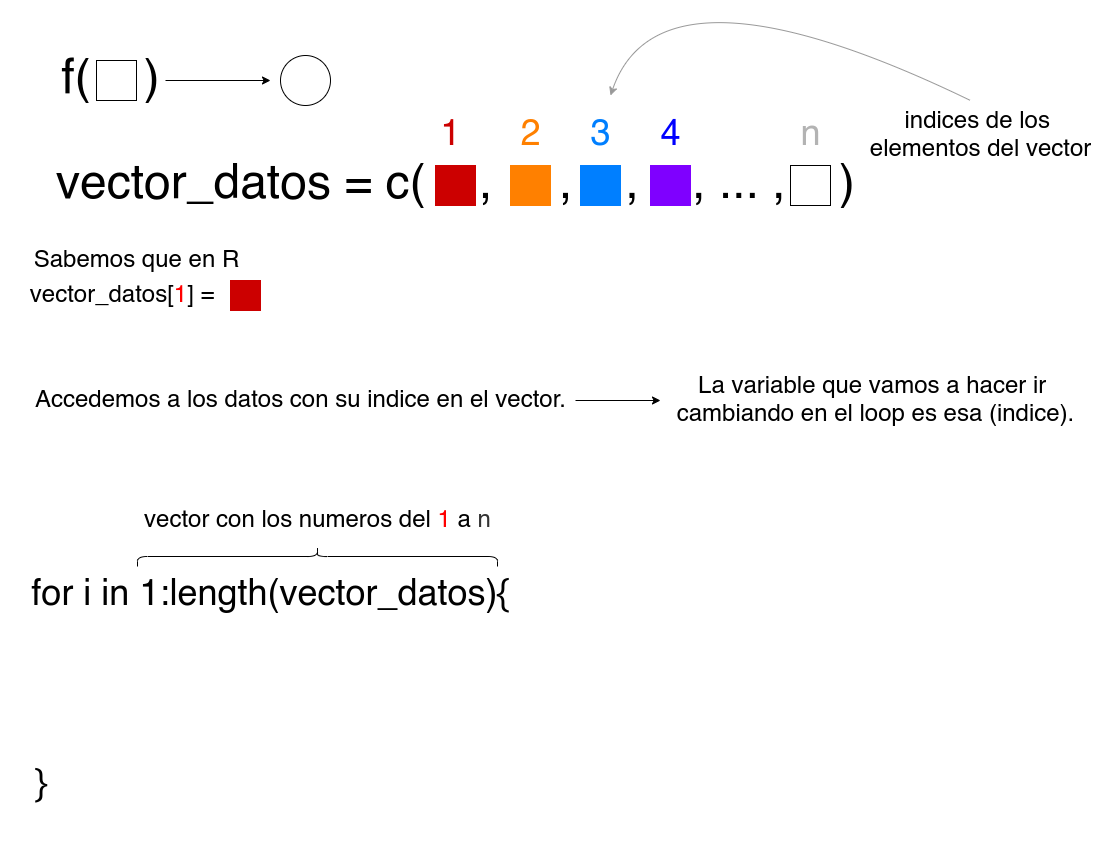
\includegraphics[width=0.9\linewidth]{images/explicando_forloops_en_r_0d} \end{center}
\end{frame}

\begin{frame}{For loop (la logica)}
\protect\hypertarget{for-loop-la-logica-4}{}
\begin{center}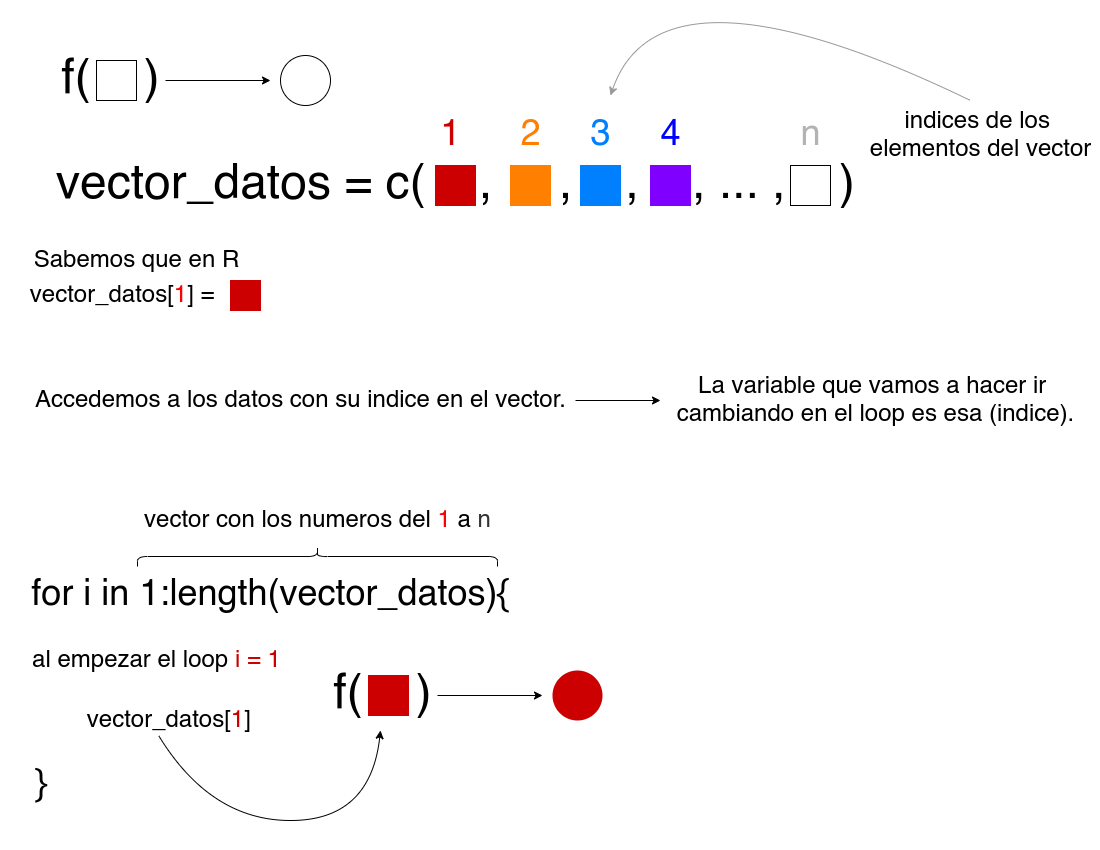
\includegraphics[width=0.9\linewidth]{images/explicando_forloops_en_r_1} \end{center}
\end{frame}

\begin{frame}{For loop (la logica)}
\protect\hypertarget{for-loop-la-logica-5}{}
\begin{center}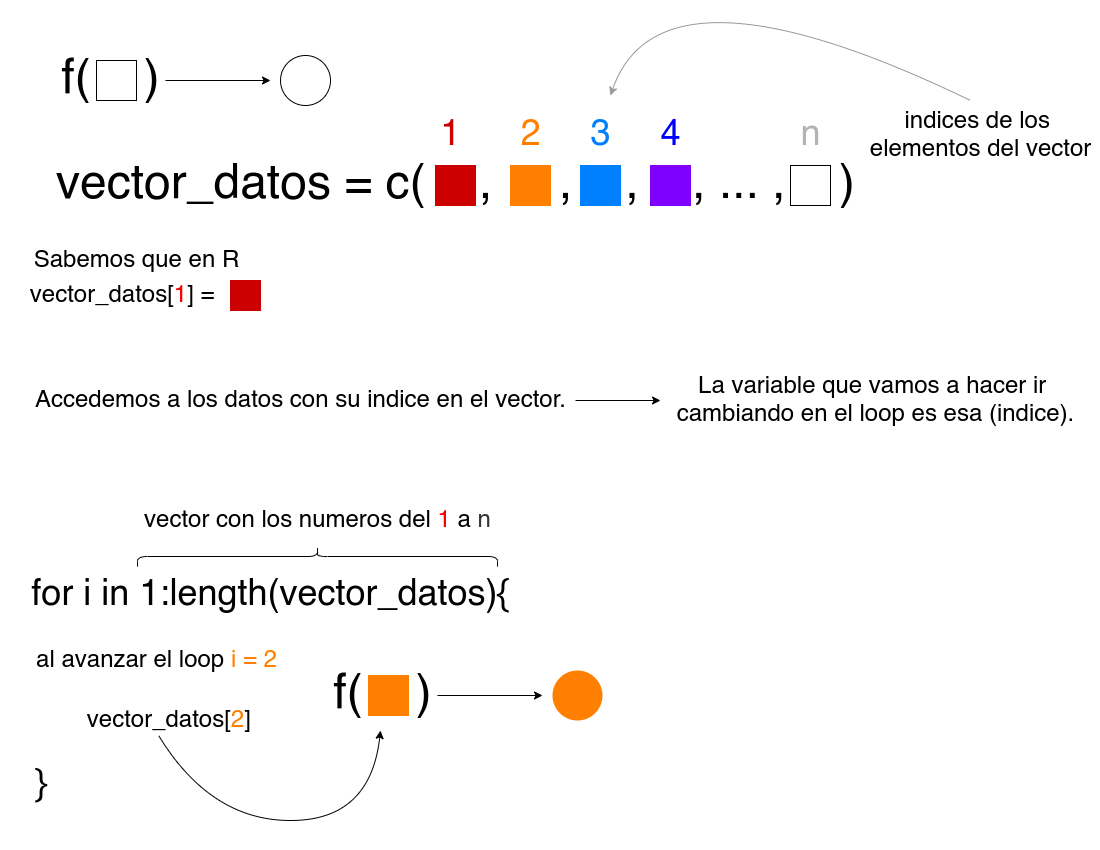
\includegraphics[width=0.9\linewidth]{images/explicando_forloops_en_r_2} \end{center}
\end{frame}

\begin{frame}{For loop (la logica)}
\protect\hypertarget{for-loop-la-logica-6}{}
\begin{center}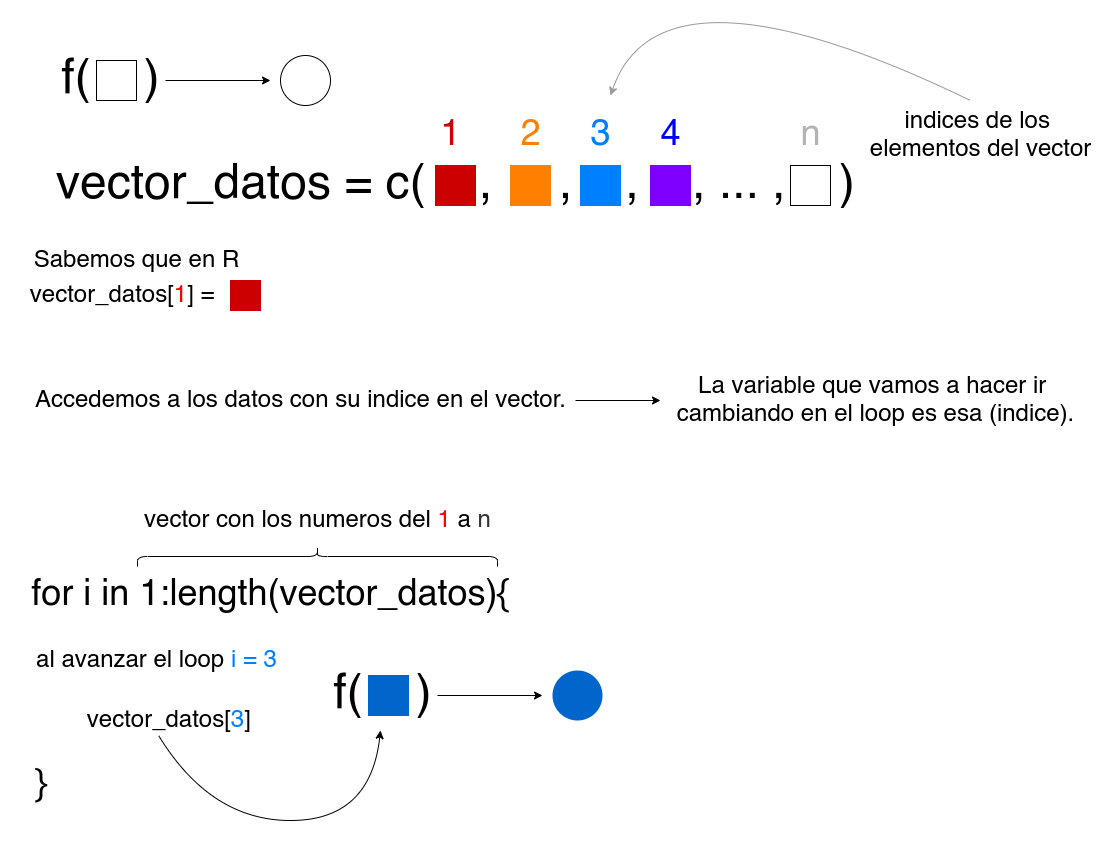
\includegraphics[width=0.9\linewidth]{images/explicando_forloops_en_r_3} \end{center}
\end{frame}

\begin{frame}[fragile]{For loop (ejemplo con codigo)}
\protect\hypertarget{for-loop-ejemplo-con-codigo}{}
\begin{Shaded}
\begin{Highlighting}[]
\NormalTok{numeros }\OtherTok{=} \FunctionTok{c}\NormalTok{(}\DecValTok{3}\NormalTok{,}\DecValTok{40}\NormalTok{,}\DecValTok{15}\NormalTok{,}\DecValTok{6}\NormalTok{)}
\NormalTok{numeros\_cuadrado }\OtherTok{=} \FunctionTok{c}\NormalTok{()}

\ControlFlowTok{for}\NormalTok{ (i }\ControlFlowTok{in} \DecValTok{1}\SpecialCharTok{:}\FunctionTok{length}\NormalTok{(numeros)) \{}
\NormalTok{  numeros\_cuadrado[i] }\OtherTok{=}\NormalTok{ numeros[i]}\SpecialCharTok{\^{}}\DecValTok{2}
\NormalTok{\}}
\end{Highlighting}
\end{Shaded}
\end{frame}

\begin{frame}[fragile]{Funciones *apply(): otra forma de \emph{loopear}}
\protect\hypertarget{funciones-apply-otra-forma-de-loopear}{}
Son \emph{funciones de alto rango}: uno de sus argumentos es otra
funcion, la cual aplican sobre un objeto.

\small

\begin{Shaded}
\begin{Highlighting}[]
\CommentTok{\# definimos un vector}
\NormalTok{numeros }\OtherTok{=} \FunctionTok{c}\NormalTok{(}\DecValTok{1}\NormalTok{,}\DecValTok{2}\NormalTok{,}\DecValTok{3}\NormalTok{,}\DecValTok{4}\NormalTok{)}

\CommentTok{\# aplicamos una funcion anonima sobre este vector}
\NormalTok{numeros\_cuadrado }\OtherTok{=} \FunctionTok{sapply}\NormalTok{(}\AttributeTok{X =}\NormalTok{ numeros, }\AttributeTok{FUN =} \ControlFlowTok{function}\NormalTok{(x)\{x}\SpecialCharTok{\^{}}\DecValTok{2}\NormalTok{\})}

\NormalTok{numeros\_cuadrado}
\end{Highlighting}
\end{Shaded}

\begin{verbatim}
## [1]  1  4  9 16
\end{verbatim}

\normalsize

\vspace{12pt}

Tenemos varias opciones, que dan diferentes clases de salidas: sapply
(vectores), lapply (listas), mapply (matrices).
\end{frame}

\hypertarget{comentarios-dudas-existenciales}{%
\section{Comentarios, dudas
existenciales?}\label{comentarios-dudas-existenciales}}

\begin{frame}{A programar se ha dicho :)}
\protect\hypertarget{a-programar-se-ha-dicho}{}
\begin{itemize}
\tightlist
\item
  10 minutos de pausa y volvemos. \vspace{20pt}
\item
  El practico de hoy esta en
  \href{https://rpubs.com/mlangleib/797813}{este link} (clickear).
\end{itemize}
\end{frame}

\end{document}
